\section{A \Cyclus Model of Nuclear Weapon Pursuit}
\label{s_methods}

We have applied the factors correlated to pursuit of nuclear weapons in a regional model of state interactions using \Cyclus\cite{huff_open_2011,huff_fundamental_2016,gidden_agent-based_2013}.  The \gls{CNERG}\footnote{http://cnerg.github.io/} group at the University of Wisconsin has developed the \Cyclus\footnote{http://fuelcycle.org/} nuclear fuel cycle simulator to model all aspects of the nuclear fuel cycle in a flexible way \cite{cyclus_v1_3}.  \Cyclus has three key features: it is \textit{agent-based}, it tracks \textit{discrete materials}, and it incorporates \textit{social and behavioral interaction models}\cite{jennings_agent-based_2000, taylor2014agent}. This design allows customized facilities and institutions to engage in dynamic decision-making based on their preferences, needs, or political constraints across a wide range of scenarios.  A specific agent might have preferences based on material composition, physical proximity between facilities, or preferred trading partners, which are implemented in a region-institution-facility hierarchy that enables economic modeling \cite{oliver_geniusv2:_2009}.
%%update cyclus_v1_3 to newer doi

\subsection{The Forward Model}

The region-institution-facility design has been used to develop the \gls{NWPM}. This forward model features two custom archetypes, an interaction region (InteractRegion) and a state institution (StateInst)\footnote{https://github.com/CNERG/mbmore}.  The state institution represents a nation-state.  It includes time-dynamic information about each of the pursuit factors. The interaction region is an omniscient presence in the simulation that tracks weapon status as well as interactive pursuit factors such as conflict (as described in section \ref{section:s_pe}), and communicates that factor to each individual state. 

Each of the motivating factors is defined for every state in a time dynamic way. Individual factors must have values between 0-10. There are several time dynamics currently available in the model: constant, linear growth or decline, step-function (at either a specified or a randomly chosen time), or power-law.  These functions enable modeling of characteristics such as growth in military spending, development of new technologies such as enrichment, and sudden changes to factors such as governing structure or inter-state conflict.  At each timestep, the state combines all of these factor values into a pursuit score using the weighted linear equation defined in section \ref{section:s_factors}.

 \subsection{Likelihood}

\begin{figure}%[htbp!]
\begin{center}
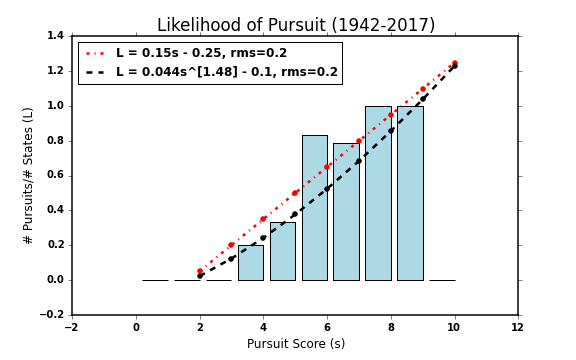
\includegraphics[scale=0.8]{./figs/pe_likely.png}
\end{center}
\caption{Fraction of states with any nuclear technology (dataset from \ref{s_factors}) that pursued weapons at some point in the last 75 years, given their pursuit scores. Although a power-law curve (black) and a weighted linear fit (red) are equivalent with the existing data, a complete set of nation-states would increase the relative weight of lower scores, making the exponential curve a better fit.}
\label{fig:likely}
\end{figure}
 
The score is then converted into a likelihood that the state will pursue a weapon. The relationship between pursuit score and likelihood of pursuing a weapon has been characterized using historical data of the 42 states that have developed nuclear technology since 1942.  \ref{fig:likely} shows the fraction of states with a given pursuit score that pursued a weapon during that time. A power-law (red) or a linear fit (black) are  equivalently valid with the 42 state dataset. However, a global dataset of nation-states would have disproportionately lower scores and zero incidences of pursuit, so we consider the power-law paramaterization to be more representative.

The data shown in \ref{fig:likely} represents the total likelihood integrated over the course of 75 years ($T$). Equation \ref{eqn:likely_eqn} is used to convert this time-integrated likelihood, $L$, into a yearly probability of pursuit, $p$.
\begin{equation}
p = 1 - (1 - L)^{1.0/T}
\label{eqn:likely_eqn}
\end{equation}

In the \gls{NWPM} forward model, each state's score is converted to time-integrated likelihood of pursuit using the power-law shown in figure \ref{fig:likely}. The actual conversion is bounded using two Heavyside functions such that scores below a lower threshold (e.g. 4) are forced to a likelihood of zero, while scores above an upper threshold (e.g. 9) are forced to the value of the score at that threshold. This is then converted to a probability at that timestep using Equation \ref{eqn:likely_eqn}   A random number generator is used with this binary probability to determine whether or not the pursuit event occurs. If the determination is for pursuit to occur, the state deploys a secret enrichment facility. If a state is already pursuing a weapon, then the model determines whether it succeeds in acquiring a weapon at that timestep using a median time to acquire of 7.5 years, based on historical data for states that have acquired weapons. On the timestep in which a state succeeds in acquiring a weapon, highly enriched uranium is shipped out of the secret enrichment facility.
% do we need to include acquisition???  I a not really happy with that model yet

% should this subsection go in the next section
\subsection{Limitations of the Historical Data and Model}
The use of historical data to develop a forward model has several limitations. The biggest limitation is in the size of this data set, both in terms of the number of countries and in the range of years that it includes.

Since the data set already includes all countries that have pursued nuclear weapons, the missing countries would only be relevant if they had pursuit scores of 4 or larger, thus reducing the time-integrated likelihood of pursuit associated with such scores. Due to the influence of nuclear technology, a non-nuclear state could theoretically have a maximum pursuit score of 7. Considering that the majority of states that have high potential military spending and major historical conflicts have already been incorporated, this further reduces the potential maximum score to below 5, even if all other factors were maximized.  A large fraction of states in the world are expected to have scores on the order of 1-3, and thus not alter the distribution shown in \ref{fig:likely}.

A more important addition to the database would be data for each country for all years between
1940 \TODO{Is ths the right year} and the year of pursuit and/or aquisition.  This would allow the direct calculation of an annual probability of pursuit as a function of the pursuit score.  The current model for converting a time-integrated likelihood to an annual probability inherently assumes that the pursuit score for the countries in the data set is constant for all the years prior to the decision to pursue nuclear weapons.  An effort fo assemble this data would be a valuable contribution to this modeling effort.

\TODO{need to place the following sentences/paragraphs in the right context}
This analysis has identified factors that are correlated to weapons programs but there is insufficient data to confirm causal relationships.   

This model is intrinsically limited by the small sample size and the degree to which the global landscape changes over time. With only 10 states that have acquired nuclear weapons throughout history, there is large uncertainty in any quantatitative analysis. Additionally, while conflict has been captured in a crude way, it is difficult to develop a parameterization with enough nuance to capture the varying impact of conflict under paradigms such as World War II, the Cold War, or post-9/11.

